\chapter{Contenido multimedia y streaming}\label{chap:5}
\section{Vídeo en la web}
\subsubsection{Ejercicio 1}
Una vez creado el \Verb#index.html#, se lanza la imagen de docker mediante el
siguiente comando:
\begin{verbatim}
docker run --rm -d --network pruebas --name nginx -p 80:80
    -v $(pwd)/html/video5/:/usr/share/nginx/html nginx
\end{verbatim}

Al acceder a \Verb#localhost:80#, se accede correctamente a la página web: \\
\begin{minipage}{\linewidth}
	\centering
	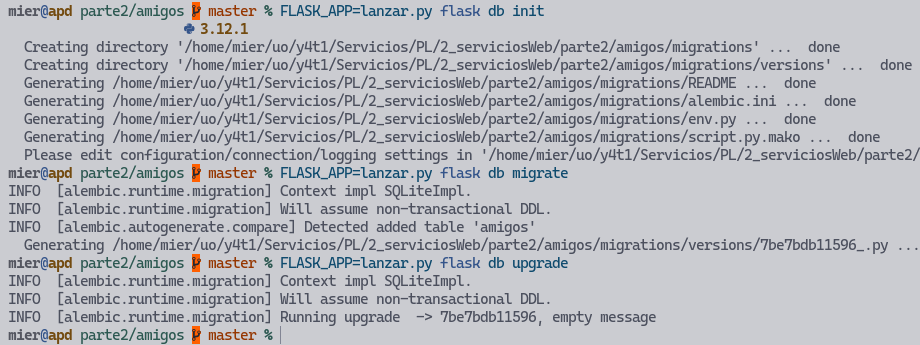
\includegraphics[width=\textwidth]{5/1.png}
	\captionof{figure}{Página web con el vídeo}\label{fig:5/1}
\end{minipage}

Mediante las herramientas de desarrollador, se aprecia que se descargan fragmentos del vídeo
según se necesiten, incluyendo las cabeceras que especifican el rango de bytes a descargar: \\
\begin{minipage}{\linewidth}
	\centering
	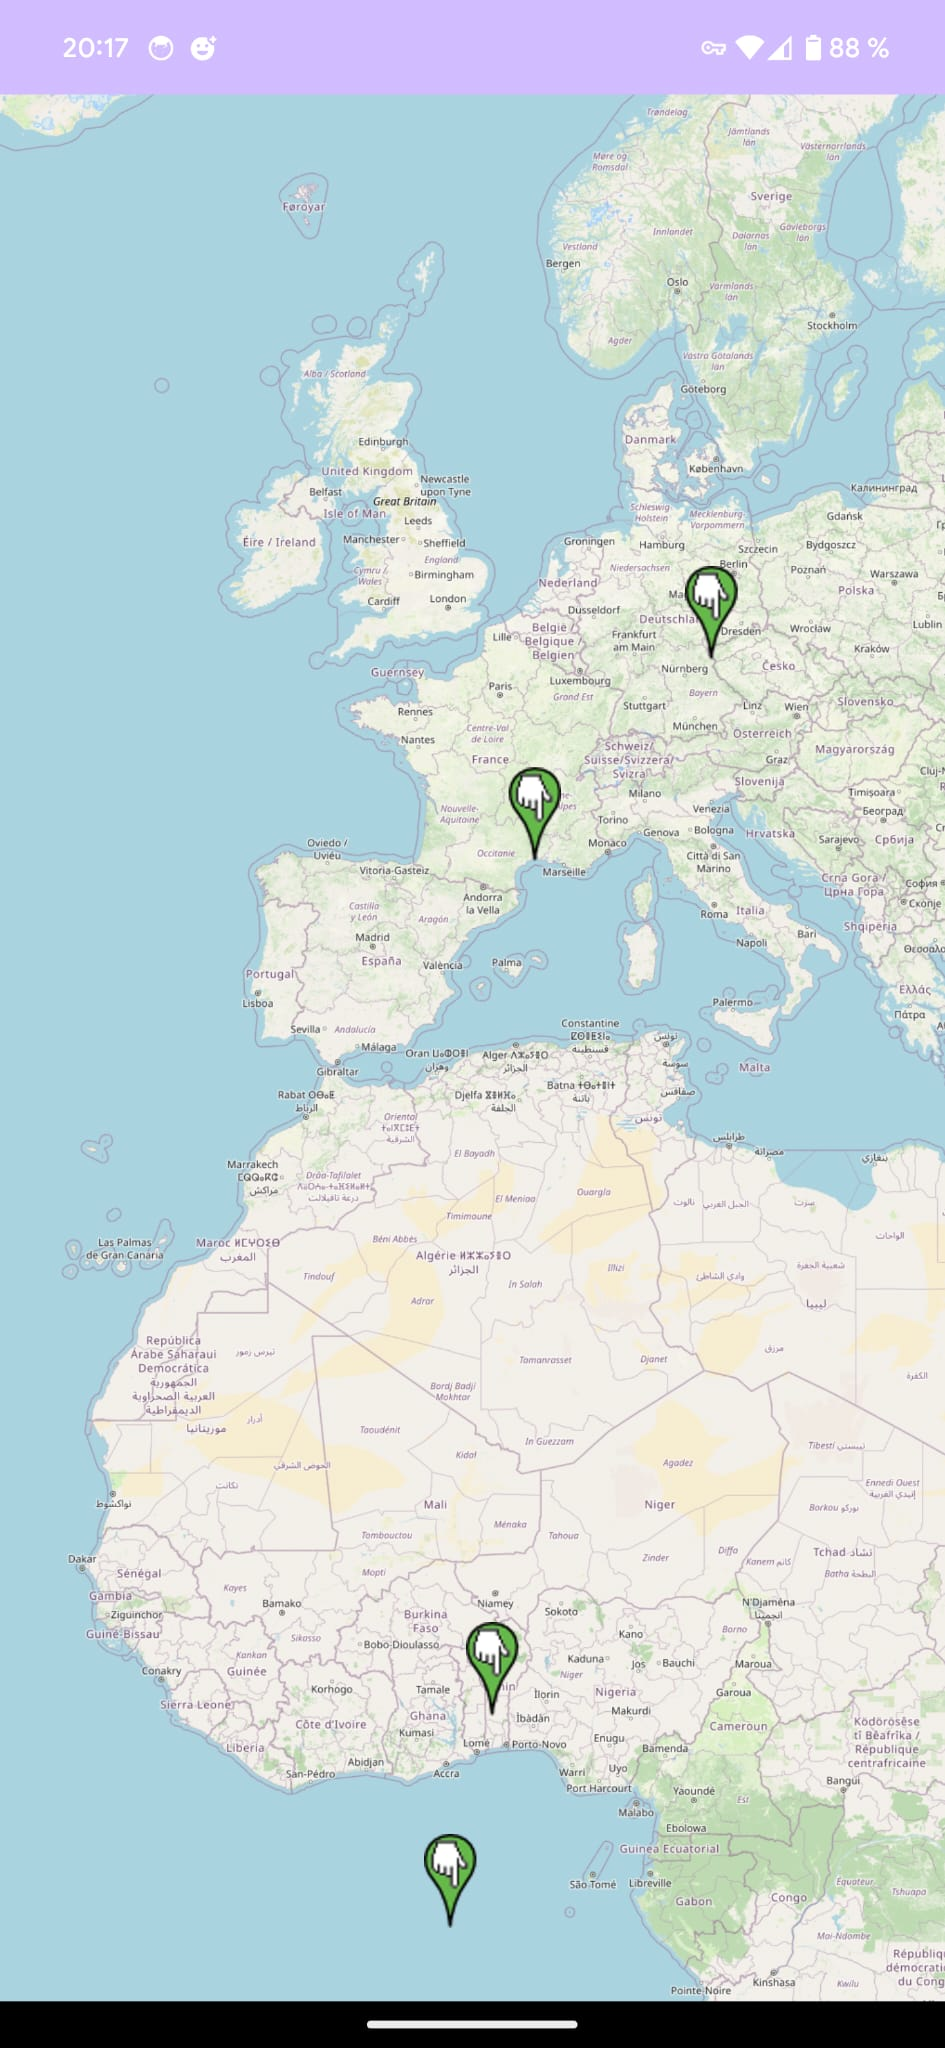
\includegraphics[width=\textwidth]{5/2.png}
	\captionof{figure}{Cabeceras de la descarga del vídeo}\label{fig:5/2}
\end{minipage}

\subsubsection{Modifica ahora la página y utiliza como fuente otro vídeo}
En mi caso, Firefox en Linux admite los tres formatos disponibles (\Verb#mp4#, \Verb#webm# y \Verb#ogv#).
|TODO| revisar

\subsubsection{Modifica la página anterior para incluir todas las fuentes disponibles}
Este ejercicio no tiene más gracia que añadir las tres fuentes disponibles en la página web,
una detrás de otra junto con un mensaje de error en caso de que no se pueda reproducir el vídeo.

\begin{verbatim}
...
<source ... type="video/ogg;  codecs...">
<source ... type="video/mp4;  codecs...">
<source ... type="video/webm; codecs...">

<object type="application/x-shockwave-flash" ...>
	...
	<!-- Fallback final: -->
	<p>No se puede reproducir el video</p>
</object>
...
\end{verbatim}

\subsubsection{Ejercicio 2~(videojs)}
Este ejercicio solo consiste en añadir al ejemplo de \Verb#videojs# las fuentes de vídeo
disponibles en el ejercicio anterior.

\begin{minipage}{\linewidth}
	\centering
	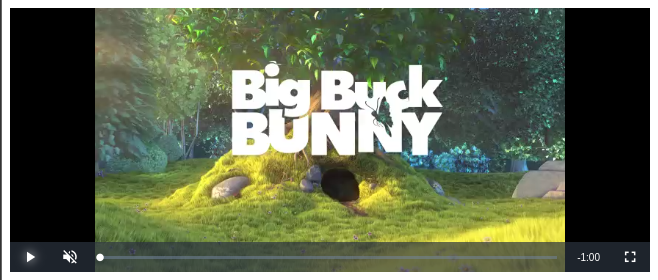
\includegraphics[width=\textwidth]{5/3.png}
	\captionof{figure}{Reproductor videojs}\label{fig:5/3}
\end{minipage}

\section{Servidor de streaming}
\subsection{Instalación de Wowza}
Durante el desarrollo de esta parte de la práctica, se hace uso del contenedor \Verb#wowza#,
que se instala con los comandos indicados en el enunciado.

\begin{minipage}{\linewidth}
	\centering
	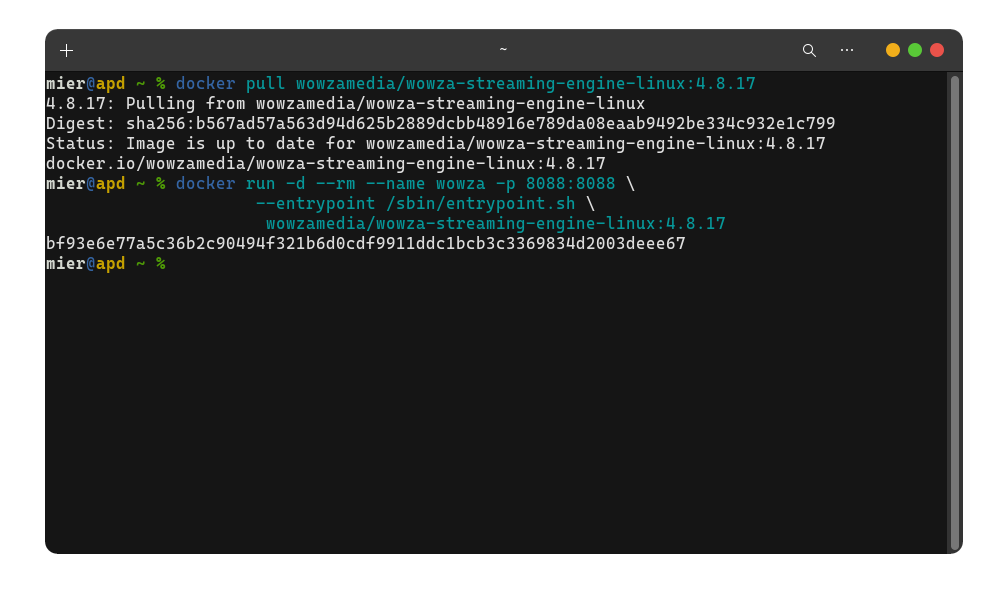
\includegraphics[width=\textwidth]{5/4.png}
	\captionof{figure}{Instalación de wowza}\label{fig:5/4}
\end{minipage}

Puesto que se está instalando directamente en la máquina física en Linux, no se necesitan
más pasos para acceder a través del navegador.

\begin{minipage}{\linewidth}
	\centering
	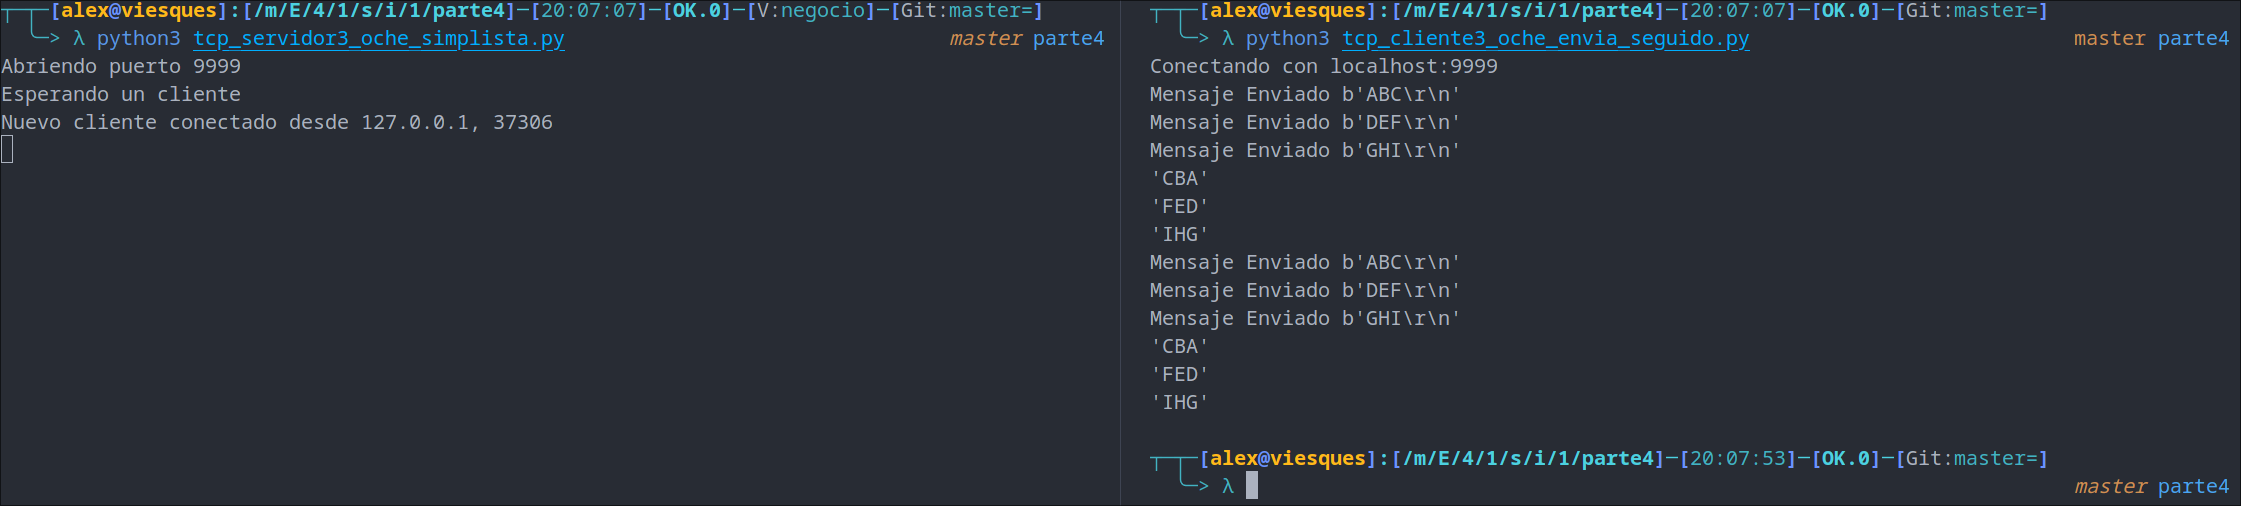
\includegraphics[width=\textwidth]{5/5.png}
	\captionof{figure}{Página de inicio de wowza}\label{fig:5/5}
\end{minipage}

Tras seguir los pasos indicados en el enunciado de creación de directorios y ficheros,
se relanza el contenedor con el siguiente comando:

\begin{minipage}{\linewidth}
	\centering
	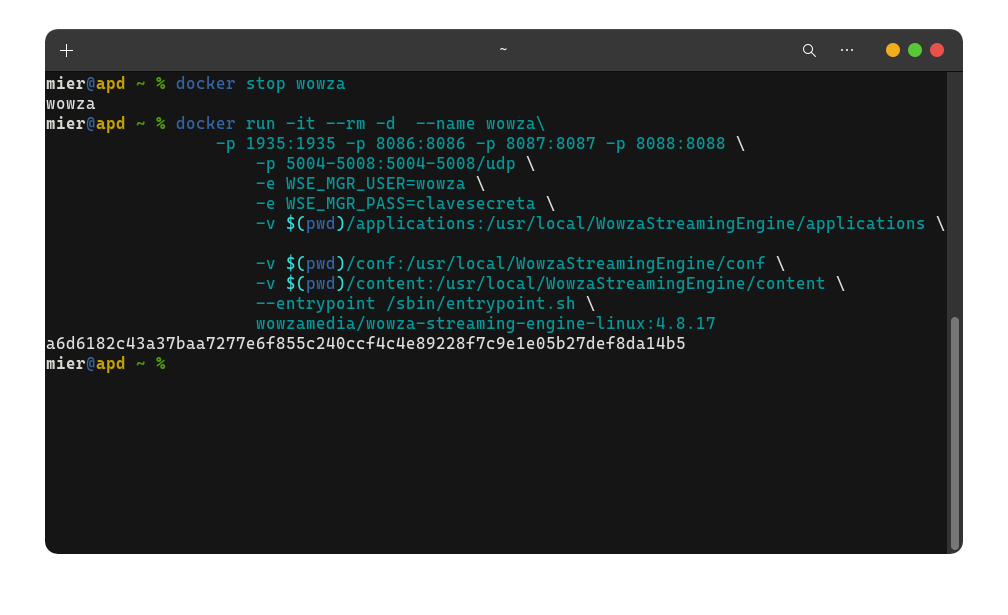
\includegraphics[width=\textwidth]{5/6.png}
	\captionof{figure}{Relanzamiento de wowza}\label{fig:5/6}
\end{minipage}

\subsection{Servicios de streaming: VOD}
Ahora, se siguen todas las instrucciones del enunciado para crear las aplicaciones
de streaming. Se crea y modifica el fichero de configuración de la aplicación
\Verb#videodemanda#. Para probarla, se utiliza la función de \Verb#Test Playback#.

\begin{minipage}{\linewidth}
	\centering
	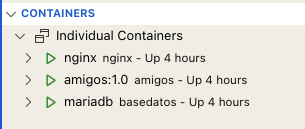
\includegraphics[width=\textwidth]{5/7.png}
	\captionof{figure}{Configuración de prueba de la aplicación videodemanda}\label{fig:5/7}
\end{minipage}

\subsubsection{Prueba de reproducción de VLC}
Para esta prueba, se hace uso del enlace \Verb#MPEG-DASH# con la función de red de VLC{.}

\begin{minipage}{\linewidth}
	\centering
	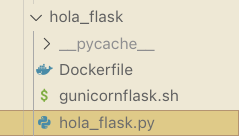
\includegraphics[width=\textwidth]{5/8.png}
	\captionof{figure}{Prueba de reproducción de VLC}\label{fig:5/8}
\end{minipage}

\subsubsection{Prueba de reproducción desde un navegador (DASH)}
Desde la página de ejemplo del consorcio MPEG-DASH, se accede a la aplicación
utilizando los enlaces \Verb#MPEG-DASH# y \Verb#HLS#.

\begin{minipage}{\linewidth}
	\centering
	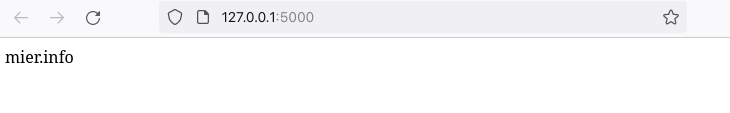
\includegraphics[width=\textwidth]{5/9.png}
	\captionof{figure}{Prueba de reproducción de MPEG-DASH}\label{fig:5/9}
\end{minipage}

\subsubsection{Escribe tu propia página con reproductor JavaScript integrado}\label{sec:5/HLS}
Tal y como dice la práctica, se crea un fichero que lea el formato HLS propietario de Apple
haciendo uso del reproductor \Verb#videojs#.

\begin{minipage}{\linewidth}
	\centering
	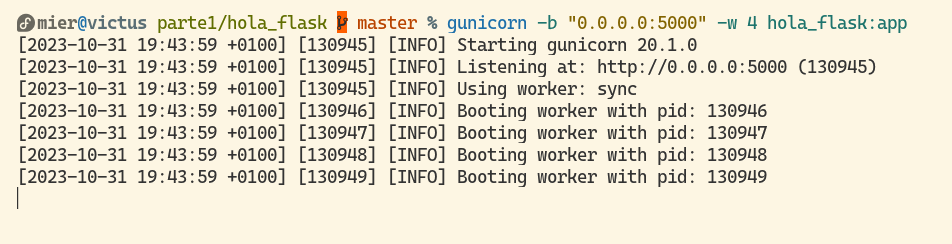
\includegraphics[width=\textwidth]{5/10.png}
	\captionof{figure}{Reproductor HLS}\label{fig:5/10}
\end{minipage}

\subsection{Servicios de streaming: streaming}
Para esta práctica, se descarga el fichero indicado y se configura VLC de forma que retransmita
a través del puerto 5004 con el protocolo RTP{.} Después, se configura como ``Incoming stream''
en la aplicación \textit{envivo} de Wowza y se comprueba que se transmite correctamente haciendo
uso del portal de MPEG-DASH visto anteriormente. En esta parte hay que hacer especial incapié en
tener cuidado con las direcciones IP, puertos y el nombre del stream, ya que un pequeño error
puede hacer que no funcione. La dirección URL resultante es la siguiente:

\begin{verbatim}
http://localhost:1935/envivo/cam.stream/manifest.mpd
\end{verbatim}

\begin{minipage}{\linewidth}
	\centering
	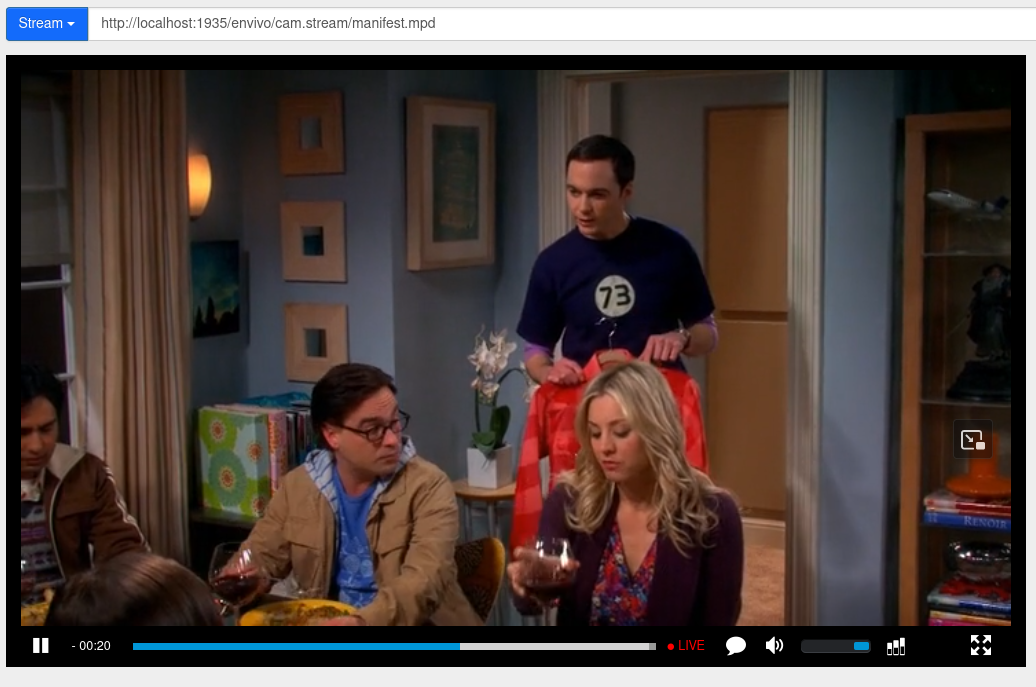
\includegraphics[width=\textwidth]{5/11.png}
	\captionof{figure}{Ejemplo de retransmisión RTP funcional}\label{fig:5/11}
\end{minipage}

\subsection{Servicios de streaming: streaming ABR}
En esta práctica, se juega con las calidades y el bitrate ``adaptativo'' a través de
\textit{smil}, un fichero de configuración que permite especificar las diferentes
calidades disponibles y el bitrate de cada una de ellas. En este caso, se ha creado
un fichero \Verb#conejo.smil# con las entradas obtenidas gracias a la herramienta
\Verb#ffprobe# del contenido descargado.

\begin{minipage}{\linewidth}
	\centering
	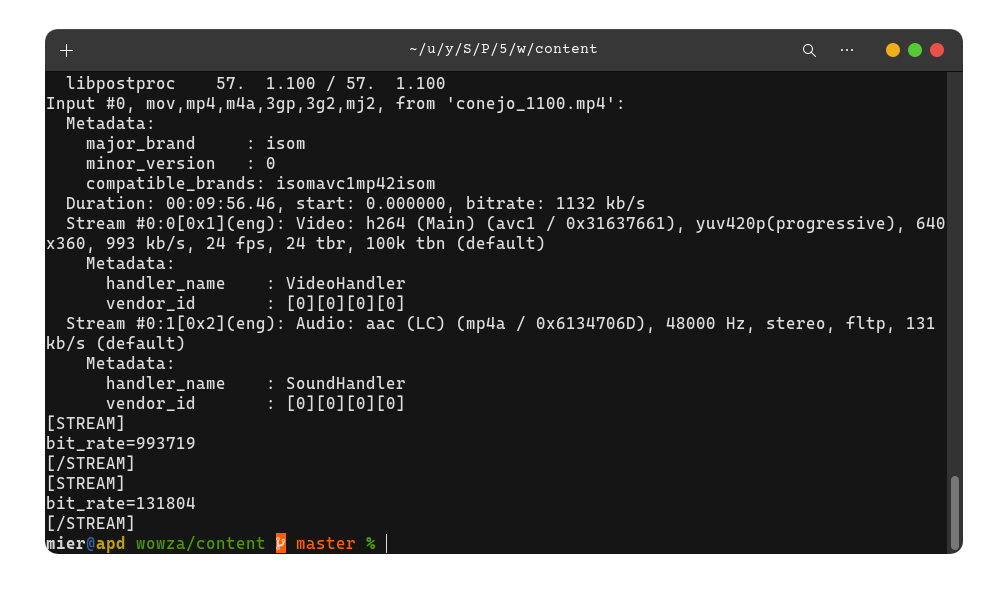
\includegraphics[width=\textwidth]{5/12.png}
	\captionof{figure}{Ejemplo de salida de ffprobe}\label{fig:5/12}
\end{minipage}

El fichero \Verb#conejo.smil# queda de la siguiente forma:

\begin{verbatim}
<video height="120" src="conejo_300.mp4" width="212">
	<param name="videoBitrate" value="170819" valuetype="data"></param>
	<param name="audioBitrate" value="131804" valuetype="data"></param>
</video>
<video height="180" src="conejo_450.mp4" width="320">
	<param name="videoBitrate" value="344453" valuetype="data"></param>
	<param name="audioBitrate" value="131804" valuetype="data"></param>
</video>
<video height="268" src="conejo_750.mp4" width="476">
	<param name="videoBitrate" value="644274" valuetype="data"></param>
	<param name="audioBitrate" value="131804" valuetype="data"></param>
</video>
<video height="360" src="conejo_1100.mp4" width="640">
	<param name="videoBitrate" value="993719" valuetype="data"></param>
	<param name="audioBitrate" value="131804" valuetype="data"></param>
</video>
\end{verbatim}

\begin{minipage}{\linewidth}
	\centering
	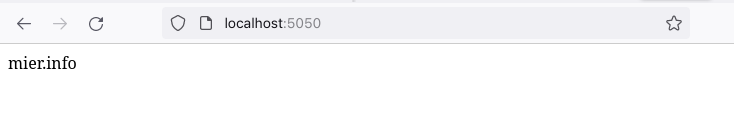
\includegraphics[width=\textwidth]{5/13.png}
	\captionof{figure}{Visualización del fichero SMIL dentro de Wowza}\label{fig:5/13}
\end{minipage}

Tras todo esto, se comprueba que funciona haciendo uso (otra vez) del mismo portal de
referencia. Como dice el enunciado, van a ocurrir errores debido a incompatibilidades
el contenido servido y el reproductor.

\begin{minipage}{\linewidth}
	\centering
	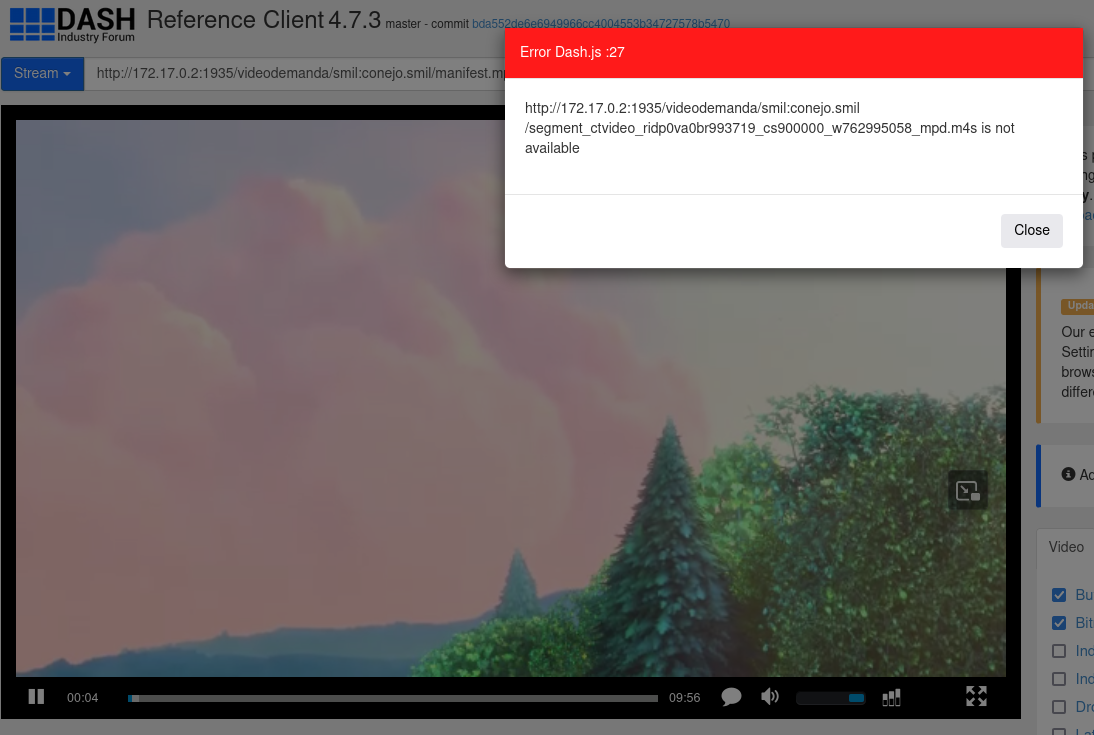
\includegraphics[width=\textwidth]{5/14.png}
	\captionof{figure}{Error en el reproductor con contenido SMIL}\label{fig:5/14}
\end{minipage}

Para probar el contenido sin erorres, se hace uso del fichero HLS que se ha creado
en la práctica anterior(Ver \ref{sec:5/HLS}). En este caso, se ha modificado el fichero \Verb#conejo.smil#
para que apunte a la dirección URL del fichero HLS{.}

\begin{minipage}{\linewidth}
	\centering
	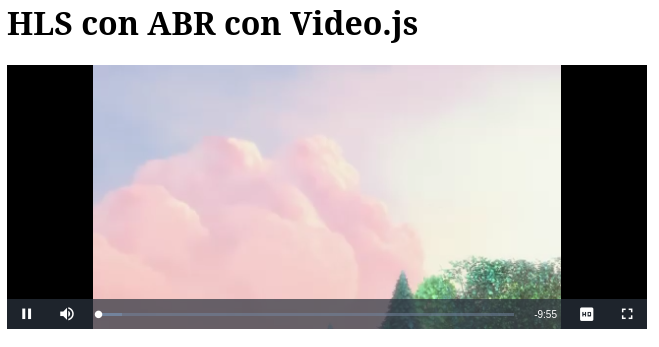
\includegraphics[width=\textwidth]{5/15.png}
	\captionof{figure}{Reproductor HLS con contenido SMIL}\label{fig:5/15}
\end{minipage}

Como se puede apreciar en la captura anterior, el reproductor incluye un selector
de calidad que no estaba disponible originalmente. Esto se consigue gracias a las
librerías indicadas que se aplican al reproductor \Verb#videojs#.

\subsubsection{Preguntas finales}
\paragraph{¿Qué bitrate ha elegido el cliente?}
Para conseguir esta información, se hace uso de las herramientas de desarrollador
de Firefox. En la pestaña de red, se puede ver el bitrate de cada una de las
descargas realizadas.

\begin{minipage}{\linewidth}
	\centering
	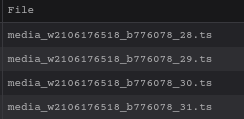
\includegraphics[width=0.5\textwidth]{5/16.png}
	\captionof{figure}{Bitrate de la descarga}\label{fig:5/16}
\end{minipage}

En este caso, se está descargando el fichero \Verb#conejo_750.mp4#, por lo que
el bitrate elegido es de 644274 bits/s (para el vídeo).

\paragraph{Si cambias el reproductor a pantalla completa durante un rato, ¿cambiará el recurso de vídeo elegido?}
Sí, después de un rato de reproducción a pantalla completa, el reproductor escoge el recurso
con calidad superior (\Verb#conejo_1100.mp4#) para reproducir el vídeo.
